\documentclass{standalone}
\usepackage{tikz}
\usetikzlibrary{patterns, positioning}
\usepackage[sfdefault]{ClearSans} %% option 'sfdefault' activates Clear Sans as the default text font
\usepackage[T1]{fontenc}

\begin{document}
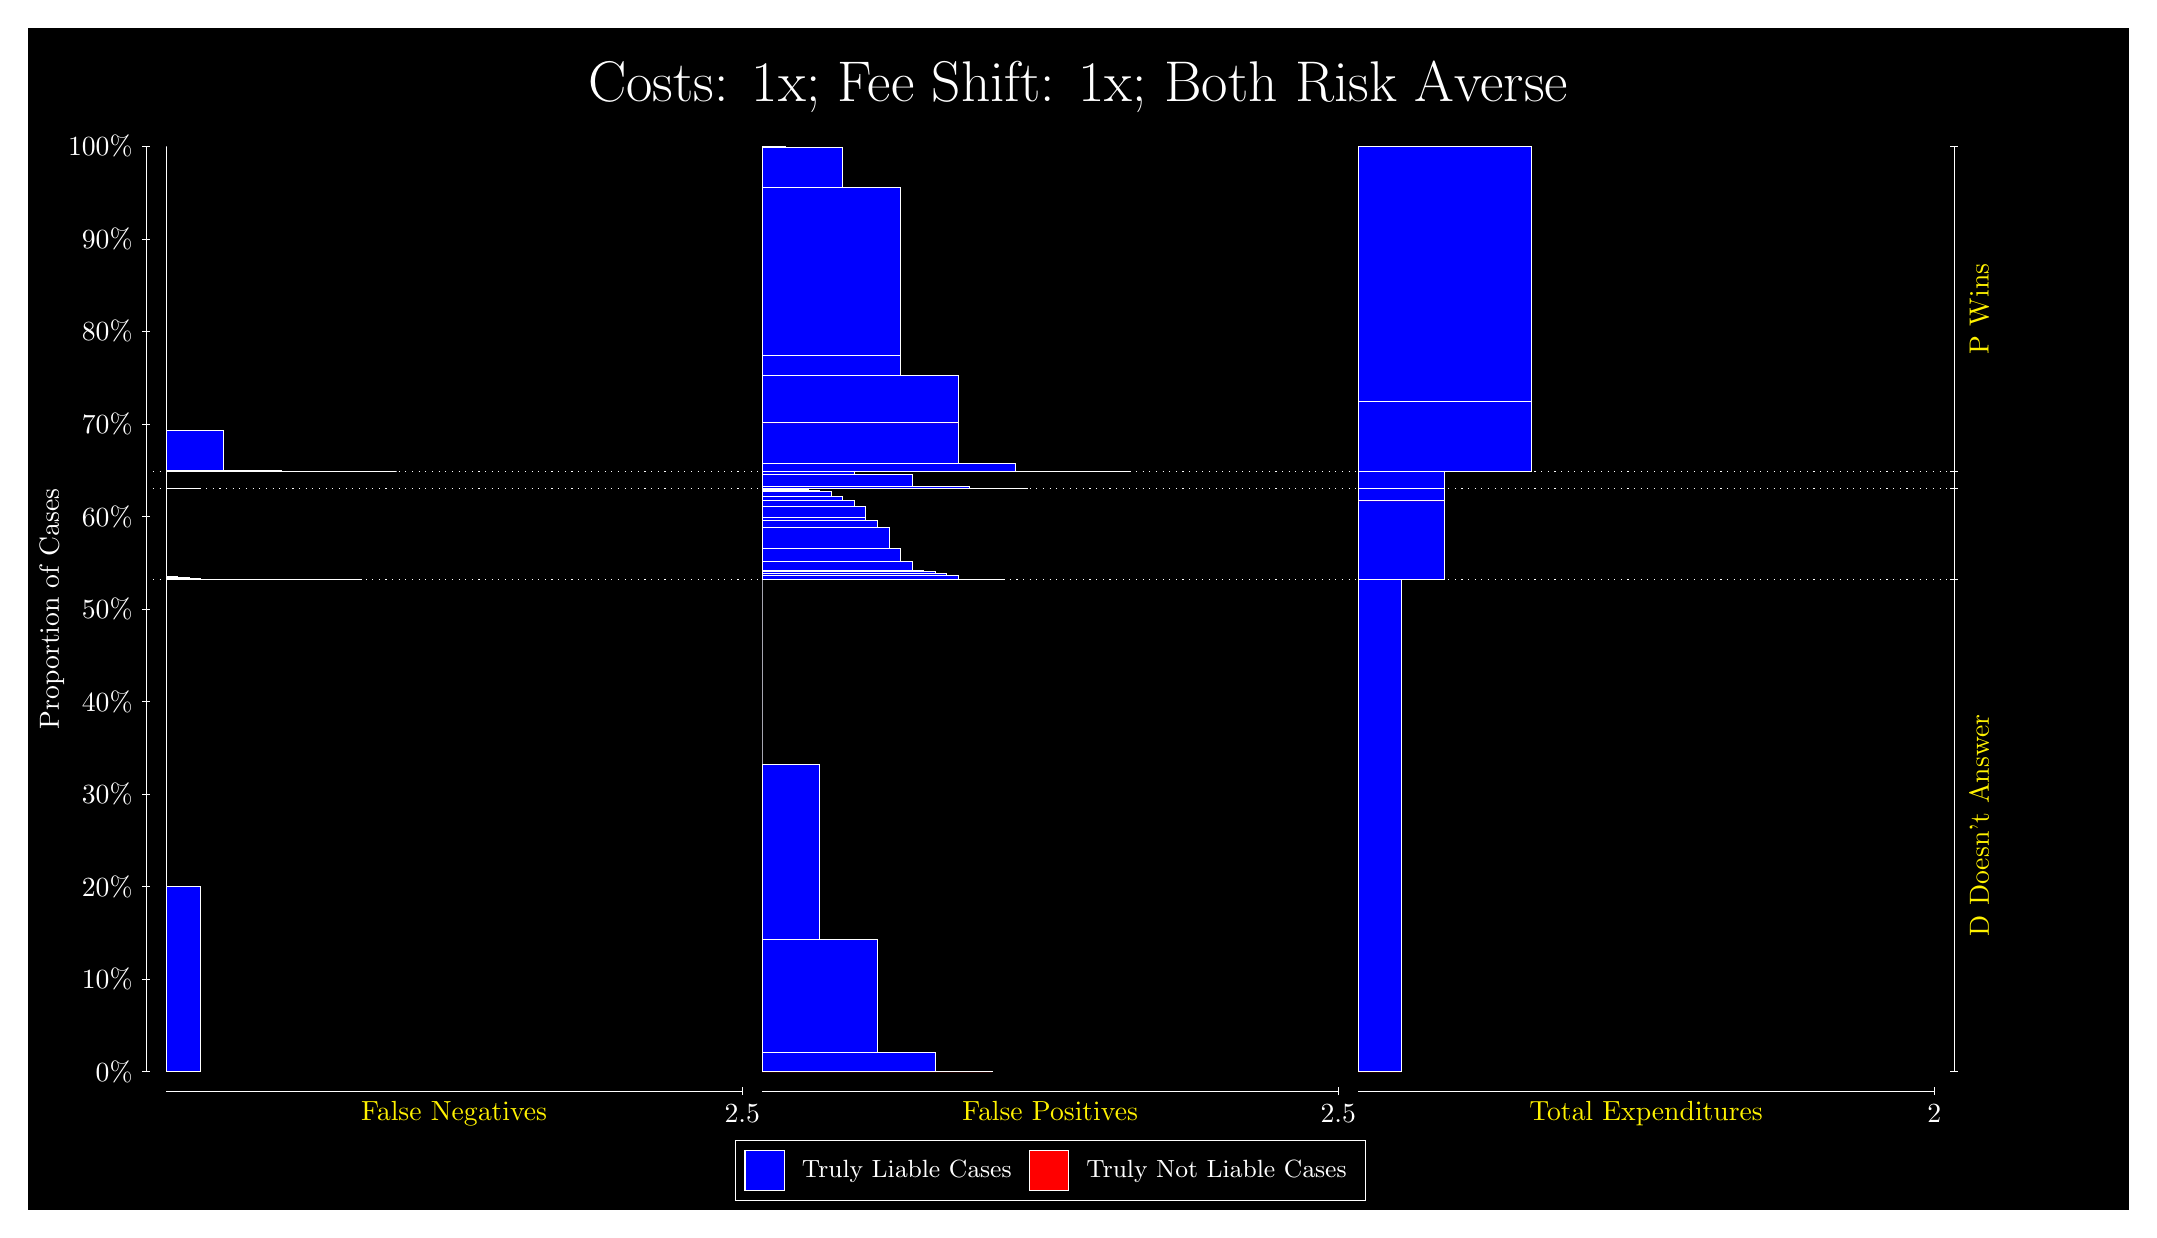
\begin{tikzpicture}
\draw[fill=black] (0,0) rectangle (26.667,15);
\draw[text=white] (0,13.5) rectangle (26.667,15) node[midway] {\huge Costs: 1x; Fee Shift: 1x; Both Risk Averse};
\draw[white, very thin] (1.5,1.75) -- (1.5,13.5);
\node[rotate=90, text=white, anchor=center] at (0.3, 7.625) {Proportion of Cases};
\draw[white, very thin] (1.45,1.75) -- (1.55,1.75);
\node[text=white, anchor=east] at (1.45, 1.75) {0\%};
\draw[white, very thin] (1.45,2.925) -- (1.55,2.925);
\node[text=white, anchor=east] at (1.45, 2.925) {10\%};
\draw[white, very thin] (1.45,4.1) -- (1.55,4.1);
\node[text=white, anchor=east] at (1.45, 4.1) {20\%};
\draw[white, very thin] (1.45,5.275) -- (1.55,5.275);
\node[text=white, anchor=east] at (1.45, 5.275) {30\%};
\draw[white, very thin] (1.45,6.45) -- (1.55,6.45);
\node[text=white, anchor=east] at (1.45, 6.45) {40\%};
\draw[white, very thin] (1.45,7.625) -- (1.55,7.625);
\node[text=white, anchor=east] at (1.45, 7.625) {50\%};
\draw[white, very thin] (1.45,8.8) -- (1.55,8.8);
\node[text=white, anchor=east] at (1.45, 8.8) {60\%};
\draw[white, very thin] (1.45,9.975) -- (1.55,9.975);
\node[text=white, anchor=east] at (1.45, 9.975) {70\%};
\draw[white, very thin] (1.45,11.15) -- (1.55,11.15);
\node[text=white, anchor=east] at (1.45, 11.15) {80\%};
\draw[white, very thin] (1.45,12.325) -- (1.55,12.325);
\node[text=white, anchor=east] at (1.45, 12.325) {90\%};
\draw[white, very thin] (1.45,13.5) -- (1.55,13.5);
\node[text=white, anchor=east] at (1.45, 13.5) {100\%};

\draw[white, very thin] (24.457,1.75) -- (24.457,13.5);
\draw[white, very thin] (24.407,1.75) -- (24.507,1.75);
\node[anchor=west] at (24.407, 1.75) {};
\draw[white, very thin] (24.407,8.004) -- (24.507,8.004);
\node[anchor=west] at (24.407, 8.004) {};
\draw[white, very thin] (24.407,9.156) -- (24.507,9.156);
\node[anchor=west] at (24.407, 9.156) {};
\draw[white, very thin] (24.407,9.3706) -- (24.507,9.3706);
\node[anchor=west] at (24.407, 9.3706) {};
\draw[white, very thin] (24.407,13.5) -- (24.507,13.5);
\node[anchor=west] at (24.407, 13.5) {};

\draw[white, very thin, fill=blue] (1.75,1.75) rectangle (2.1891,4.0987);
\draw[white, very thin, fill=red] (1.75,4.0987) rectangle (1.75,4.0987);
\draw[white, very thin, fill=blue] (1.75,4.0987) rectangle (1.75,8.004);
\draw[white, very thin, fill=blue] (1.75,8.004) rectangle (4.2384,8.004);
\draw[white, very thin, fill=blue] (1.75,8.004) rectangle (3.9457,8.004);
\draw[white, very thin, fill=blue] (1.75,8.004) rectangle (3.6529,8.004);
\draw[white, very thin, fill=blue] (1.75,8.004) rectangle (3.5065,8.004);
\draw[white, very thin, fill=blue] (1.75,8.004) rectangle (3.3602,8.004);
\draw[white, very thin, fill=blue] (1.75,8.004) rectangle (3.2138,8.004);
\draw[white, very thin, fill=blue] (1.75,8.004) rectangle (3.0674,8.004);
\draw[white, very thin, fill=blue] (1.75,8.004) rectangle (2.921,8.004);
\draw[white, very thin, fill=blue] (1.75,8.004) rectangle (2.7746,8.004);
\draw[white, very thin, fill=blue] (1.75,8.004) rectangle (2.6283,8.0041);
\draw[white, very thin, fill=blue] (1.75,8.0041) rectangle (2.4819,8.0047);
\draw[white, very thin, fill=blue] (1.75,8.0047) rectangle (2.3355,8.0058);
\draw[white, very thin, fill=blue] (1.75,8.0058) rectangle (2.1891,8.0104);
\draw[white, very thin, fill=blue] (1.75,8.0104) rectangle (2.0428,8.0276);
\draw[white, very thin, fill=blue] (1.75,8.0276) rectangle (2.0428,8.0293);
\draw[white, very thin, fill=blue] (1.75,8.0293) rectangle (1.8964,8.0381);
\draw[white, very thin, fill=red] (1.75,8.0381) rectangle (1.75,8.0381);
\draw[white, very thin, fill=blue] (1.75,8.0381) rectangle (1.75,9.156);
\draw[white, very thin, fill=blue] (1.75,9.156) rectangle (2.1891,9.1564);
\draw[white, very thin, fill=red] (1.75,9.1564) rectangle (1.75,9.1564);
\draw[white, very thin, fill=blue] (1.75,9.1564) rectangle (1.75,9.3706);
\draw[white, very thin, fill=blue] (1.75,9.3706) rectangle (4.6775,9.3706);
\draw[white, very thin, fill=blue] (1.75,9.3706) rectangle (3.9457,9.3706);
\draw[white, very thin, fill=blue] (1.75,9.3706) rectangle (3.2138,9.3824);
\draw[white, very thin, fill=blue] (1.75,9.3824) rectangle (2.4819,9.8955);
\draw[white, very thin, fill=red] (1.75,9.8955) rectangle (1.75,9.8955);
\draw[white, very thin, fill=blue] (1.75,9.8955) rectangle (1.75,13.5);
\draw[white, very thin, fill=red] (9.3189,1.75) rectangle (12.246,1.75);
\draw[white, very thin, fill=blue] (9.3189,1.75) rectangle (12.246,1.7525);
\draw[white, very thin, fill=blue] (9.3189,1.7525) rectangle (11.515,2.0004);
\draw[white, very thin, fill=blue] (9.3189,2.0004) rectangle (10.783,3.4339);
\draw[white, very thin, fill=blue] (9.3189,3.4339) rectangle (10.051,5.6553);
\draw[white, very thin, fill=blue] (9.3189,5.6553) rectangle (9.3189,8.004);
\draw[white, very thin, fill=red] (9.3189,8.004) rectangle (12.393,8.004);
\draw[white, very thin, fill=blue] (9.3189,8.004) rectangle (12.393,8.0041);
\draw[white, very thin, fill=red] (9.3189,8.0041) rectangle (12.1,8.0041);
\draw[white, very thin, fill=blue] (9.3189,8.0041) rectangle (12.1,8.0042);
\draw[white, very thin, fill=red] (9.3189,8.0042) rectangle (11.807,8.0042);
\draw[white, very thin, fill=blue] (9.3189,8.0042) rectangle (11.807,8.0535);
\draw[white, very thin, fill=blue] (9.3189,8.0535) rectangle (11.661,8.0782);
\draw[white, very thin, fill=red] (9.3189,8.0782) rectangle (11.515,8.0782);
\draw[white, very thin, fill=blue] (9.3189,8.0782) rectangle (11.515,8.104);
\draw[white, very thin, fill=blue] (9.3189,8.104) rectangle (11.368,8.1198);
\draw[white, very thin, fill=red] (9.3189,8.1198) rectangle (11.222,8.1198);
\draw[white, very thin, fill=blue] (9.3189,8.1198) rectangle (11.222,8.2247);
\draw[white, very thin, fill=blue] (9.3189,8.2247) rectangle (11.075,8.4015);
\draw[white, very thin, fill=red] (9.3189,8.4015) rectangle (10.929,8.4015);
\draw[white, very thin, fill=blue] (9.3189,8.4015) rectangle (10.929,8.6631);
\draw[white, very thin, fill=blue] (9.3189,8.6631) rectangle (10.783,8.7458);
\draw[white, very thin, fill=blue] (9.3189,8.7458) rectangle (10.636,8.7894);
\draw[white, very thin, fill=red] (9.3189,8.7894) rectangle (10.636,8.7894);
\draw[white, very thin, fill=blue] (9.3189,8.7894) rectangle (10.636,8.9265);
\draw[white, very thin, fill=blue] (9.3189,8.9265) rectangle (10.49,9.0016);
\draw[white, very thin, fill=blue] (9.3189,9.0016) rectangle (10.344,9.0573);
\draw[white, very thin, fill=blue] (9.3189,9.0573) rectangle (10.197,9.1218);
\draw[white, very thin, fill=blue] (9.3189,9.1218) rectangle (10.051,9.1306);
\draw[white, very thin, fill=blue] (9.3189,9.1306) rectangle (9.9044,9.1323);
\draw[white, very thin, fill=blue] (9.3189,9.1323) rectangle (9.9044,9.1495);
\draw[white, very thin, fill=blue] (9.3189,9.1495) rectangle (9.758,9.1541);
\draw[white, very thin, fill=blue] (9.3189,9.1541) rectangle (9.6116,9.1553);
\draw[white, very thin, fill=blue] (9.3189,9.1553) rectangle (9.4652,9.1558);
\draw[white, very thin, fill=blue] (9.3189,9.1558) rectangle (9.3189,9.156);
\draw[white, very thin, fill=red] (9.3189,9.156) rectangle (12.686,9.156);
\draw[white, very thin, fill=blue] (9.3189,9.156) rectangle (12.686,9.1562);
\draw[white, very thin, fill=blue] (9.3189,9.1562) rectangle (11.954,9.1836);
\draw[white, very thin, fill=blue] (9.3189,9.1836) rectangle (11.222,9.3318);
\draw[white, very thin, fill=blue] (9.3189,9.3318) rectangle (10.49,9.3702);
\draw[white, very thin, fill=blue] (9.3189,9.3702) rectangle (9.758,9.3706);
\draw[white, very thin, fill=red] (9.3189,9.3706) rectangle (14.003,9.3706);
\draw[white, very thin, fill=blue] (9.3189,9.3706) rectangle (14.003,9.3706);
\draw[white, very thin, fill=red] (9.3189,9.3706) rectangle (13.271,9.3706);
\draw[white, very thin, fill=blue] (9.3189,9.3706) rectangle (13.271,9.3724);
\draw[white, very thin, fill=red] (9.3189,9.3724) rectangle (12.539,9.3724);
\draw[white, very thin, fill=blue] (9.3189,9.3724) rectangle (12.539,9.4792);
\draw[white, very thin, fill=blue] (9.3189,9.4792) rectangle (11.807,9.9922);
\draw[white, very thin, fill=red] (9.3189,9.9922) rectangle (11.807,9.9922);
\draw[white, very thin, fill=blue] (9.3189,9.9922) rectangle (11.807,10.587);
\draw[white, very thin, fill=blue] (9.3189,10.587) rectangle (11.075,10.849);
\draw[white, very thin, fill=red] (9.3189,10.849) rectangle (11.075,10.849);
\draw[white, very thin, fill=blue] (9.3189,10.849) rectangle (11.075,12.975);
\draw[white, very thin, fill=blue] (9.3189,12.975) rectangle (10.344,12.984);
\draw[white, very thin, fill=blue] (9.3189,12.984) rectangle (10.344,13.488);
\draw[white, very thin, fill=blue] (9.3189,13.488) rectangle (9.6116,13.488);
\draw[white, very thin, fill=blue] (9.3189,13.488) rectangle (9.6116,13.5);
\draw[white, very thin, fill=blue] (9.3189,13.5) rectangle (9.3189,13.5);
\draw[white, very thin, fill=red] (16.888,1.75) rectangle (17.437,1.75);
\draw[white, very thin, fill=blue] (16.888,1.75) rectangle (17.437,8.004);
\draw[white, very thin, fill=red] (16.888,8.004) rectangle (17.986,8.004);
\draw[white, very thin, fill=blue] (16.888,8.004) rectangle (17.986,9.0016);
\draw[white, very thin, fill=red] (16.888,9.0016) rectangle (17.986,9.0016);
\draw[white, very thin, fill=blue] (16.888,9.0016) rectangle (17.986,9.156);
\draw[white, very thin, fill=red] (16.888,9.156) rectangle (17.986,9.156);
\draw[white, very thin, fill=blue] (16.888,9.156) rectangle (17.986,9.3706);
\draw[white, very thin, fill=red] (16.888,9.3706) rectangle (19.083,9.3706);
\draw[white, very thin, fill=blue] (16.888,9.3706) rectangle (19.083,10.263);
\draw[white, very thin, fill=red] (16.888,10.263) rectangle (19.083,10.263);
\draw[white, very thin, fill=blue] (16.888,10.263) rectangle (19.083,13.5);
\draw[white, dotted] (1.5,8.004) -- (24.457,8.004);
\draw[white, dotted] (1.5,9.156) -- (24.457,9.156);
\draw[white, dotted] (1.5,9.3706) -- (24.457,9.3706);
\draw[white, very thin] (1.75,1.5) -- (9.0689,1.5);
\node[text=yellow, anchor=north] at (5.4094, 1.5) {False Negatives};
\draw[white, very thin] (9.0689,1.45) -- (9.0689,1.55);
\node[text=white, anchor=north] at (9.0689, 1.45) {2.5};

\draw[white, very thin] (9.3189,1.5) -- (16.638,1.5);
\node[text=yellow, anchor=north] at (12.978, 1.5) {False Positives};
\draw[white, very thin] (16.638,1.45) -- (16.638,1.55);
\node[text=white, anchor=north] at (16.638, 1.45) {2.5};

\draw[white, very thin] (16.888,1.5) -- (24.207,1.5);
\node[text=yellow, anchor=north] at (20.547, 1.5) {Total Expenditures};
\draw[white, very thin] (24.207,1.45) -- (24.207,1.55);
\node[text=white, anchor=north] at (24.207, 1.45) {2};

\node[text=yellow, centered, rotate=90] at (24.777, 4.877) {D Doesn't Answer};


\node[text=yellow, centered, rotate=90] at (24.777, 11.435) {P Wins};

\draw (12.978300999999998,1.5) node[draw=none] (baseCoordinate) {};
\begin{scope}[align=center]
        \matrix[scale=0.5, draw=white, below=0.5cm of baseCoordinate, nodes={draw}, column sep=0.1cm]{
            \node[rectangle, draw, minimum width=0.5cm, minimum height=0.5cm, fill=blue] {}; &
            \node[draw=none, font=\small, text=white] (B) {Truly Liable Cases}; &
            \node[rectangle, draw, minimum width=0.5cm, minimum height=0.5cm, fill=red] {}; &
            \node[draw=none, font=\small, text=white] (B) {Truly Not Liable Cases}; \\
            };
\end{scope}

\end{tikzpicture}
\end{document}